\documentclass{article}
\usepackage{tikz}
\renewcommand*\familydefault{\sfdefault}
\usepackage[american]{circuitikz}

\begin{document}
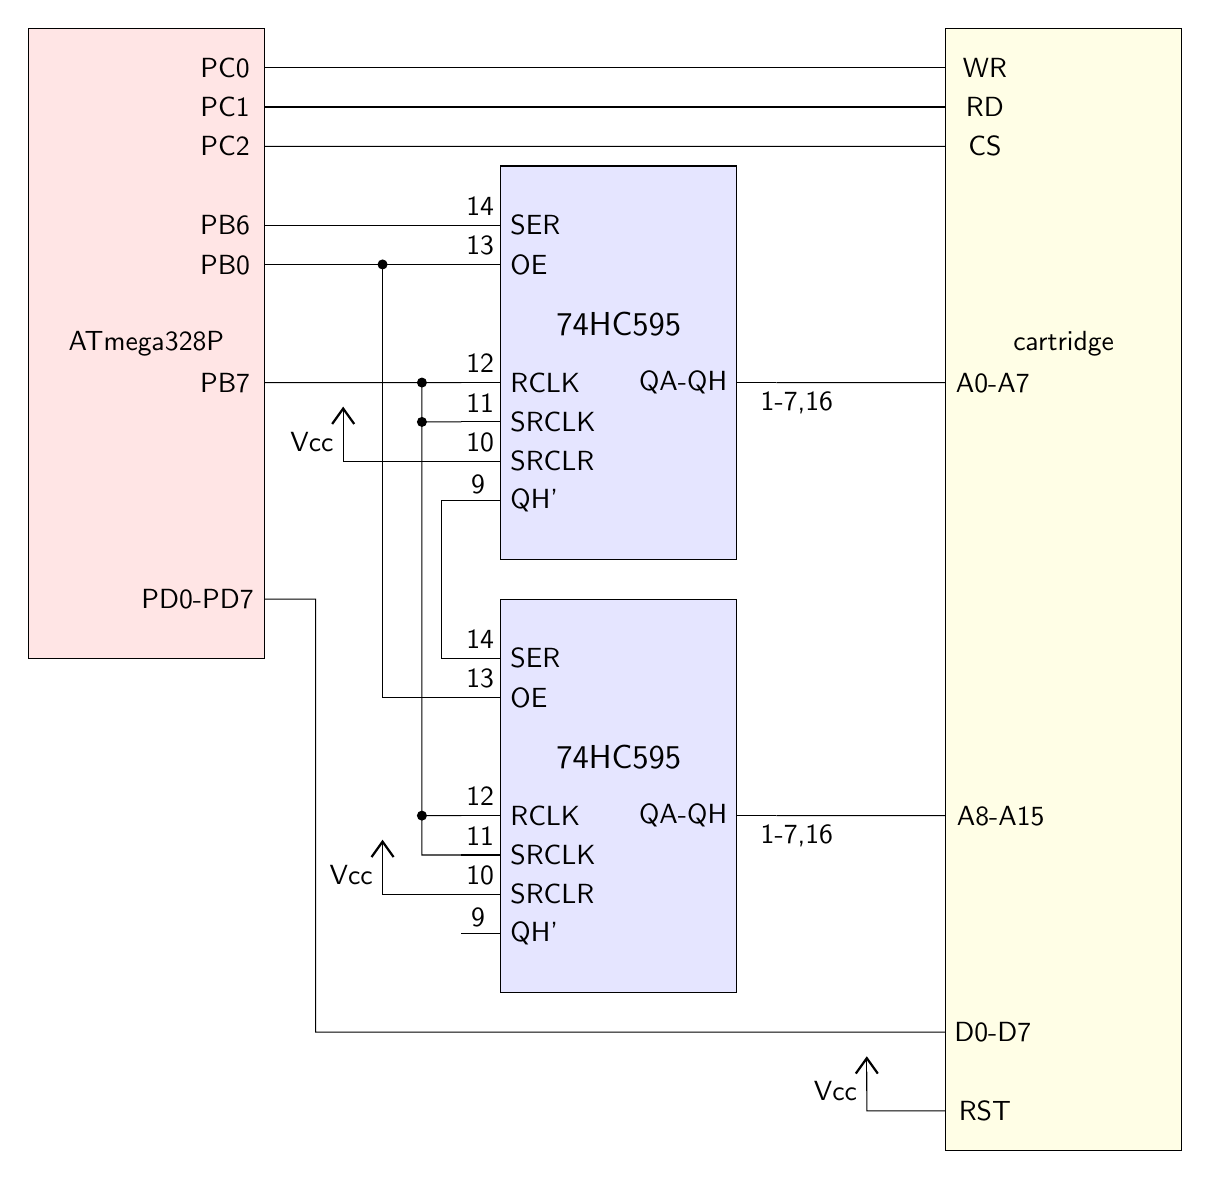
\begin{tikzpicture}
% Variables: 1 := position, 2 := ID.
\def\74xx595(#1)#2{
    \begin{scope}[shift={(#1)}]
        \draw[fill=blue!10] (-1.5, -2.5) rectangle (1.5, 2.5);
        \draw (0,0.5) node [align=center]{\large 74HC595};
        \draw (-1.5,1.75) node [right]{SER} -- +(-0.5,0) node [anchor=-135]{14} coordinate (#2 SER);
        \draw (-1.5,1.25) node [right]{OE} -- +(-0.5,0) node [anchor=-135]{13} coordinate (#2 OE);
        \draw (-1.5,-0.25) node [right]{RCLK} -- +(-0.5,0) node [anchor=-135]{12} coordinate (#2 RCLK);
        \draw (-1.5,-0.75) node [right]{SRCLK} -- +(-0.5,0) node [anchor=-135]{11} coordinate (#2 SRCLK);
        \draw (-1.5,-1.25) node [right]{SRCLR} -- +(-0.5,0) node [anchor=-135]{10} coordinate (#2 SRCLR);
        \draw (-1.5,-1.75) node [right]{QH'} -- +(-0.5,0) node [anchor=-135]{9} coordinate (#2 QH');
        \draw (1.5,-0.25) node [left]{QA-QH} -- +(0.5,0) node [anchor=135]{1-7,16} coordinate (#2 QA-QH);
    \end{scope}
}
\74xx595(0,0){1}
\74xx595(0,-5.5){2}
\draw(1 QH')
    to [short] ++(-0.25,0)
    to [short] ($ (2 SER) - (0.25,0) $)
    to [short] (2 SER);
\draw(1 RCLK)
    to [short, -*] ++(-0.5,0) coordinate (CLK)
    to [short, -*]($ (1 SRCLK) - (0.5,0) $) coordinate (TEMP)
    to [short] (1 SRCLK)
    to [short] (TEMP)
    to [short, -*] ($ (2 RCLK) - (0.5,0) $) coordinate (TEMP)
    to [short] (2 RCLK)
    to [short] (TEMP)
    to [short] ($ (2 SRCLK) - (0.5,0) $)
    to [short] (2 SRCLK);
\draw(1 OE)
    to [short, -*] ++(-1.0,0) coordinate (OE)
    to [short] ($ (2 OE) - (1.0,0) $)
    to [short] (2 OE);
\draw(1 SRCLR)
    to [short] ++(-1.50,0)
    to node[vcc,label=left:Vcc]{} ++(0,0.5);
\draw(2 SRCLR)
    to [short] ++(-1.0,0)
    to node[vcc,label=left:Vcc]{} ++(0,0.5);
\draw(CLK)
    to [short] ++(-2.0,0) coordinate (CLK);
\draw(1 SER)
    to [short] ++(-2.5,0) coordinate (SER);
\draw(OE)
    to [short] ++(-1.5,0) coordinate (OE);
\draw[fill=red!10]($ (1 SER) + (-5.5,2.5) $) coordinate (ATMEGA1) rectangle ++(3.0, -8.0) coordinate (ATMEGA2);
\draw($ (ATMEGA1) + (3,-0.5) $) coordinate (PC0)
    to [short] ++(0.65,0)
    to [short] ++(8,0) coordinate (WR);
\draw($ (ATMEGA1) + (3,-1) $) coordinate (PC1)
    to [short] ++(0.65,0)
    to [short] (WR |- PC1) coordinate (RD);
\draw($ (ATMEGA1) + (3,-1.5) $) coordinate (PC2)
    to [short] ++(0.65,0)
    to [short] (WR |- PC2) coordinate (CS);
\draw($ (ATMEGA2) + (0,0.75) $) coordinate (PORTD)
    to [short] ++(0.65,0)
    to [short] ++(0,-5.5)
    to [short] ++(8,0) coordinate (D0-D7);
\draw[fill=yellow!10]($ (WR) + (0,0.5) $) coordinate (CART1) rectangle ($ (D0-D7) + (3.0,-1.5) $) coordinate (CART2);
\draw(1 QA-QH) to [short] (CART1 |- 1 QA-QH) coordinate (A0-A7);
\draw(2 QA-QH) to [short] (CART1 |- 2 QA-QH) coordinate (A8-A15);
\draw($ (CART1 |- CART2) + (0,0.5) $)
    to [short] ++(-1.0,0)
    to node[vcc,label=left:Vcc]{} ++(0,0.5);

\node[] at ($ (SER) - (0.5,0) $) {PB6};
\node[] at ($ (CLK) - (0.5,0) $) {PB7};
\node[] at ($ (OE) - (0.5,0) $) {PB0};
\node[] at ($ (PORTD) - (0.85,0) $) {PD0-PD7};
\node[] at ($ (PC0) - (0.5,0) $) {PC0};
\node[] at ($ (PC1) - (0.5,0) $) {PC1};
\node[] at ($ (PC2) - (0.5,0) $) {PC2};
\node[] at ($ (WR) + (0.5,0) $) {WR};
\node[] at ($ (RD) + (0.5,0) $) {RD};
\node[] at ($ (CS) + (0.5,0) $) {CS};
\node[] at ($ (A0-A7) + (0.6,0) $) {A0-A7};
\node[] at ($ (A8-A15) + (0.7,0) $) {A8-A15};
\node[] at ($ (D0-D7) + (0.6,0) $) {D0-D7};
\node[] at ($ (CART1 |- CART2) + (0.5,0.5) $) {RST};
\node[] at ($ (ATMEGA1) + (1.5,-4.0) $) {ATmega328P};
\node[] at ($ (CART1) + (1.5,-4.0) $) {cartridge};
\end{tikzpicture}
\end{document}
